%%%%%%%%%%%%%%%%%%%%%%%%%%%%%%%%%%%%%%%%%%%%%%%%%%%%%%%%%%%%%%%%%
%%% COSYNE-2007 Abstract Template
%%% Version 1.0
%%%%%%%%%%%%%%%%%%%%%%%%%%%%%%%%%%%%%%%%%%%%%%%%%%%%%%%%%%%%%%%%%
% \newcommand\mybibname{New Title}
% \renewcommand\bibsection{%
%    \clearpage
%    \noindent\normalsize\MakeUppercase{\mybibname}%
%    \markboth{\MakeUppercase{\mybibname}}{\MakeUppercase{\mybibname}}%
%   }
\documentclass[12pt]{article}
\usepackage{times}
\usepackage{graphicx}
\usepackage[export]{adjustbox}
\usepackage{wrapfig}
% \usepackage{caption}
\usepackage[font=normal]{subcaption}
\usepackage{subcaption}

\def\bibfont{\footnotesize}
\renewcommand*{\bibfont}{\footnotesize}
% \renewcommand*{\bibfont}{\small}


\oddsidemargin 0.0in		% margin, in addition to 1" standard
\textwidth 6.5in		% 8.5" - 2*(1+\oddsidemargin)

% \topmargin -0.25in		% in addition to 1.5" standard margin
\topmargin -0.5in		% in addition to 1.5" standard margin
\textheight 9.25in 		% 11 - ( 1.5 + \topmargin + <bottom-margin> )
% \bottom-margin -1.0in
\columnsep 0.25in

\parindent 0pt
\parskip 12pt

\flushbottom \sloppy
\pagestyle{empty}		% No page numbers


\begin{document}

%%%----------------------------------------------------------------- 
{\bf  
An Oscillatory Neural Network model of motor system dynamics during continuous periodic movements
}

{\bf
% Ir\'{a}n Rom\'{a}n$^1$, Wisam Reid$^1$, \& Takako Fujioka$^1$ 
Ir\'{a}n Rom\'{a}n, Wisam Reid \& Takako Fujioka 
}

% {
% $^1$Stanford University
% }

%%%----------------------------------------------------------------- 

{\bf Abstract}\\
\noindent
Coordinated neural computations underlying voluntary movements are reflected in oscillatory activity. Computations in the basal ganglia (BG) are modulated by dopaminergic neurons upon the initiation of movement at the motor cortex (MC). In Parkinson's disease (PD), dopaminergic activity at the BG is low, impairing voluntary movements. Brain oscillations arise from computations between BG and MC. In PD, excessive beta-band ($\sim$ 20Hz) activity is constantly present in BG and MC, and is associated with anti-kinesis. In healthy individuals, high-gamma ($\sim$ 80Hz) bursts project from MC to BG and are associated with desynchronization of beta-band and initiation of movement. Recent computational work focuses on directional connectivity within BG nuclei. However, models have not yet explained gamma- and beta-band dynamics related to periodic movements. We implement a non-linear oscillatory neural network (ONN) to explain the coupled activity between MC and BG during periodic movement. The building block is a canonical neural oscillator at a Hopf bifurcation, allowing for abrupt, qualitative changes in dynamics. Our model has two neural oscillators, one at the high-gamma-band in a double-limit cycle, and one at the beta-band in a limit cycle. This simulates a short-burst in the former and spontaneous and continuous idling in the latter. A MC impulse drives the high-gamma oscillator, whose activity is inhibitory input to the beta-band oscillator. Periodic MC impulses are input to the network, producing bursts of gamma-band activity that suppress beta-band amplitude. This reproduces beta and high-gamma oscillations reported in healthy human electrophysiology during periodic motion. After an interval of periodic MC impulses, a memory state in our model allows the beta-band oscillator to recover its limit cycle amplitude at the point where the next impulse is anticipated. If the inhibition from gamma- to beta-band is reduced, PD activity emerges, capturing weakened dopaminergic neurons giving rise to excessive beta-band in BG and MC.  
% Our model captures oscillatory brain activity, reported in human electrophysiology literature, as triggered by periodic voluntary movements in healthy individuals and patients affected by Parkinsonism.

% The full text of the abstract, including any equations, tables, and
% figures, should appear here.  Left  margin is 1 inch (2.54 cm), and
% text width is 6.75 inches (16.5 cm), which leaves a 1 inch right
% margin on U.S.-letter sized paper.  Text is full-justified (i.e., both
% right and left side are aligned).

% Paragraphs should be separated by a blank line, and the first line 
% should not be indented.  
{\bf Methods}\\
\noindent
We build a model using nonlinear neural oscillators described by the ordinary differential equation: 

\begin{equation}
\dot{z} = z\bigg( \alpha + i\omega +\beta_1|z_i|^2+\frac{\epsilon\beta_2|z_i|^4}{1-\epsilon|z_i|^2}\bigg) + x(t)
\end{equation}

% \begin{wrapfigure}{R}{0.5\textwidth}
% \centering
% \includegraphics[width=0.4\textwidth,right]{model1.png}
% \caption{\label{fig:arch}System dynamics with isochronous stimulation}
% \end{wrapfigure}

where $x(t)$ is the input to the oscillator, $z(t)$ is a complex state variable containing amplitude and phase information ($z = re^{i\phi}$), $\omega$ is the natural frequency of oscillation, and the parameters that determine the dynamical properties of the oscillator are $\alpha$, $\beta_1$, $\beta_2$, and $\epsilon$ 
$\mathbf{[1]}\mathbf{[2]}$.
% \cite{large2010canonical}\cite{largekim2015}. 
In our model, the high-gamma oscillator receives MC impulses as input. The parameters of the high-gamma oscillator are $\alpha = -15$, $\beta_1 = 1$, $\beta_2 = -1$, and $\epsilon = 1$, which make it be a double-limit cycle oscillator capable of achieving a memory state that reflects the period of isochronous stimulation. The beta oscillator receives inhibitory input from the gamma oscillator and has parameters $\alpha = 8$, $\beta_1 = -2000$, $\beta_2 = 0$, and $\epsilon = 0$, which pose it at a limit cycle that spontaneously oscillates. \\Figure (a) shows an schematic of our model's architecture.

% This equation is referred to as a normal form because of the expansion of the nonlinearities, the higher order terms (h.o.t.). From \cite{large2010canonical}, we have  a fully expanded canonical model of a neural oscillator as:

% generic equation describing a Hopf bifurcation can be written

% \begin{equation}
% \dot{z_i} = z_i\big( \alpha + i\omega_0+(\beta_i + i\delta_i)|z_i|^2) + \mbox{h.o.t.}
% \end{equation}



% \begin{equation}
% \dot{z_i} = z_i\big( \alpha + i\omega_o +(\beta_i + i\delta_i)|z_i|^2+\frac{\epsilon(\beta_2+i\delta_2)|z_i|^4}{1-\epsilon|z_i|^2}\big) + RT
% \end{equation}

% Here we have added a quintic term by summing over a Taylor series expansion of the h.o.t.

% {\bf Results\\}
% \begin{wrapfigure}{R}{0.5\textwidth}
% \centering
% 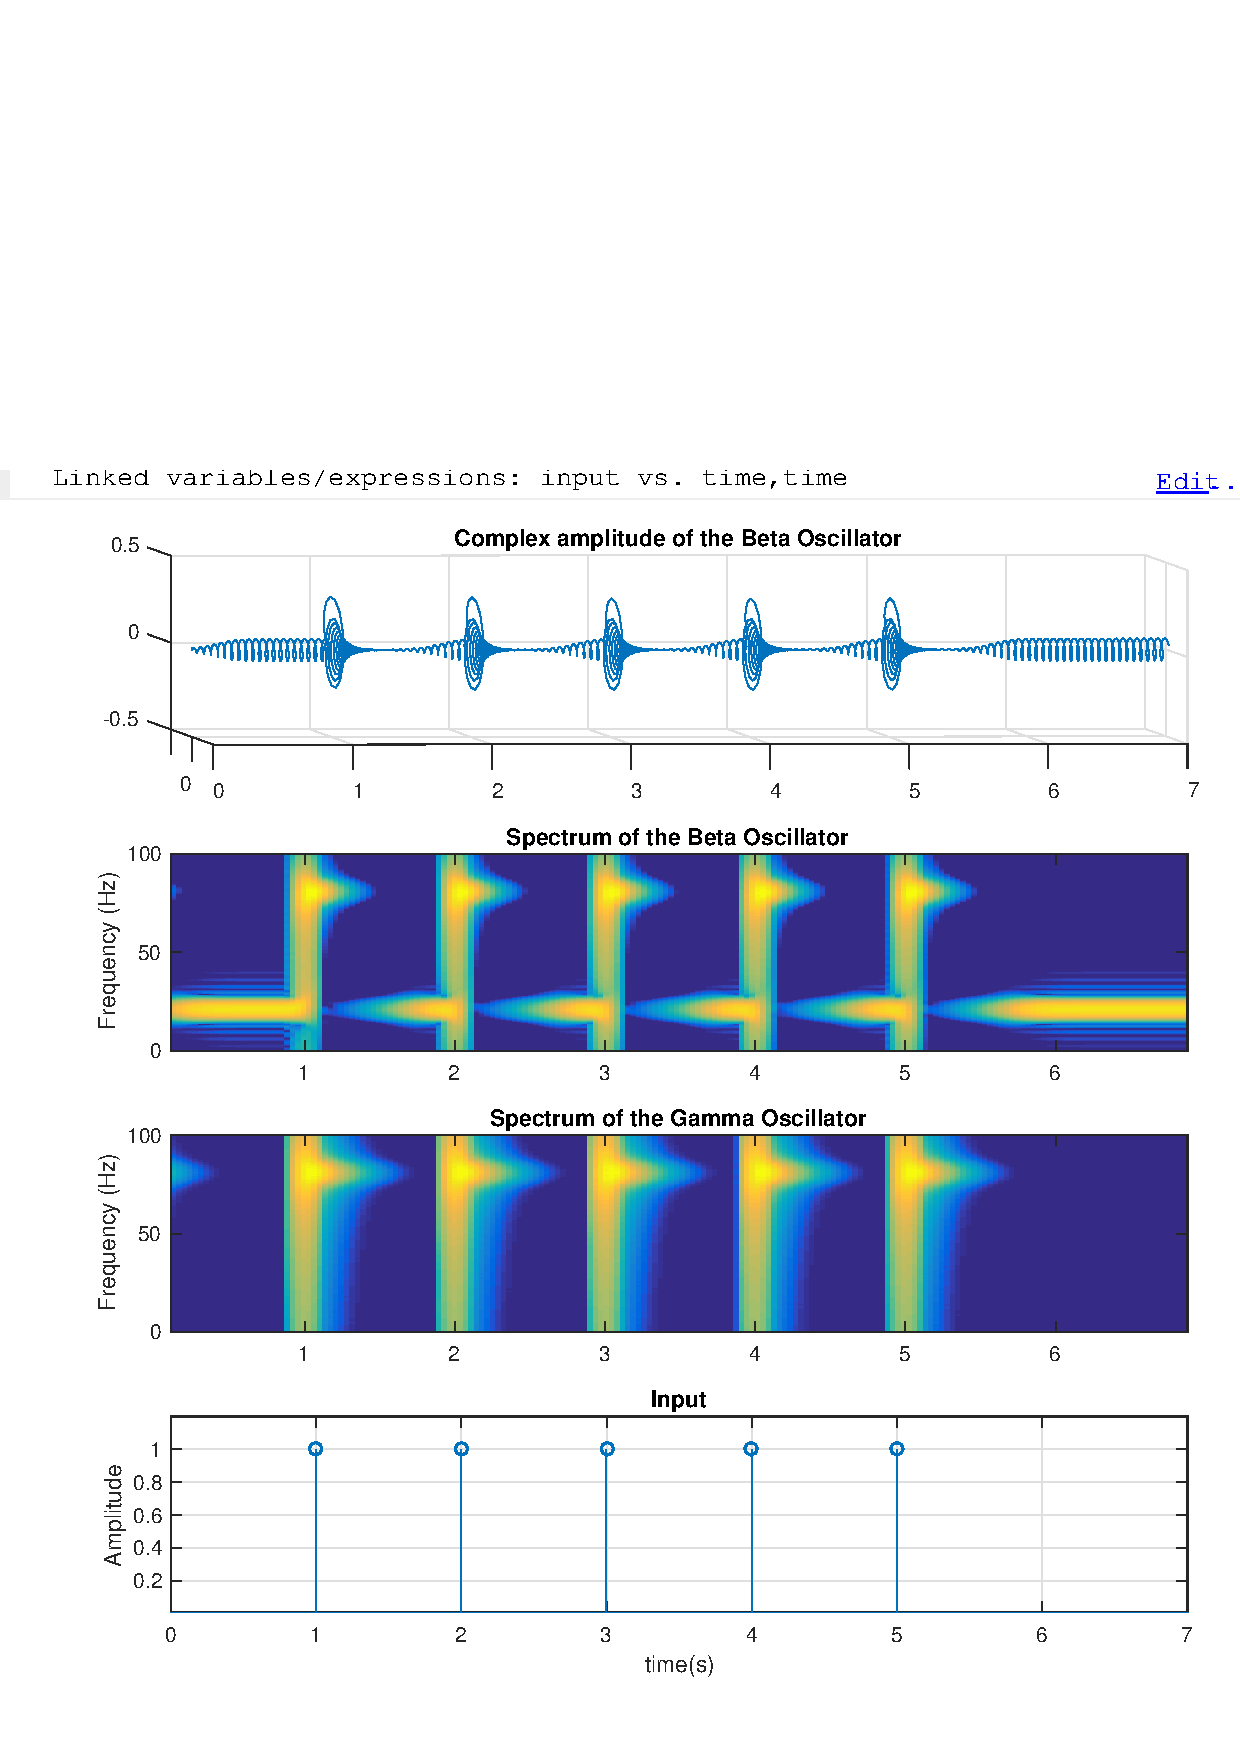
\includegraphics[width=0.5\textwidth,right]{iso_stim.png}
% \caption{\label{fig:system}System dynamics with isochronous stimulation}
% \end{wrapfigure}

\clearpage

{\bf Results}\\
\noindent
Figure (b) shows the behavior of our model through a brief period of isochronous MC impulses. The top two rows show the complex amplitude response and the spectogram, respectively, of the beta oscillator. The beta oscillator changes in amplitude upon receiving inhibitory input from the high-gamma oscillator, whose spectrogram is shown in the third row of figure (b). The MC impulses, input to the high-gamma oscillator, are shown in the bottom row of figure (b). 

{\bf Discussion}\\
\noindent
Our results are consistent with evidence from electrophysiology indicating that isochronous motion and sensory stimulation trigger a high-gamma burst, and a subsequent event related desynchronization of beta-band oscillations $\mathbf{[3][4]}$.
% \cite{fujioka2009beta} \cite{large2015neural}. 
Our model attains a memory state that reflects the period of the MC impulses, indicated by resynchronization of the beta-band to its limit cycle amplitude in anticipation of the next MC impulse. Moreover, a weakened connection from the gamma- to beta-band oscillator results in continuous beta-band activity. This weakened connection is analogous to low dopamine levels in BG nuclei, as observed in Parkinsonism $\mathbf{[5]}$.
% \cite{thompson2014clinical}.
% \cite{fujioka2009beta} \cite{pavlides2015computational}\cite{tachibana2011subthalamo} \cite{nevado2011bifurcation}

\begin{figure}
    \centering
    \begin{subfigure}[t]{0.35\textwidth}
        \includegraphics[width=\textwidth]{model1}
        \caption{ONN Architecture: [A] Output [B] MC/BG beta band [C] MC gamma bursting [D] MC impulse}
        \label{fig:arch}
    \end{subfigure}
    ~ %add desired spacing between images, e. g. ~, \quad, \qquad, \hfill etc. 
      %(or a blank line to force the subfigure onto a new line)
    \quad \quad \quad \quad
    \begin{subfigure}[t]{0.41\textwidth}
        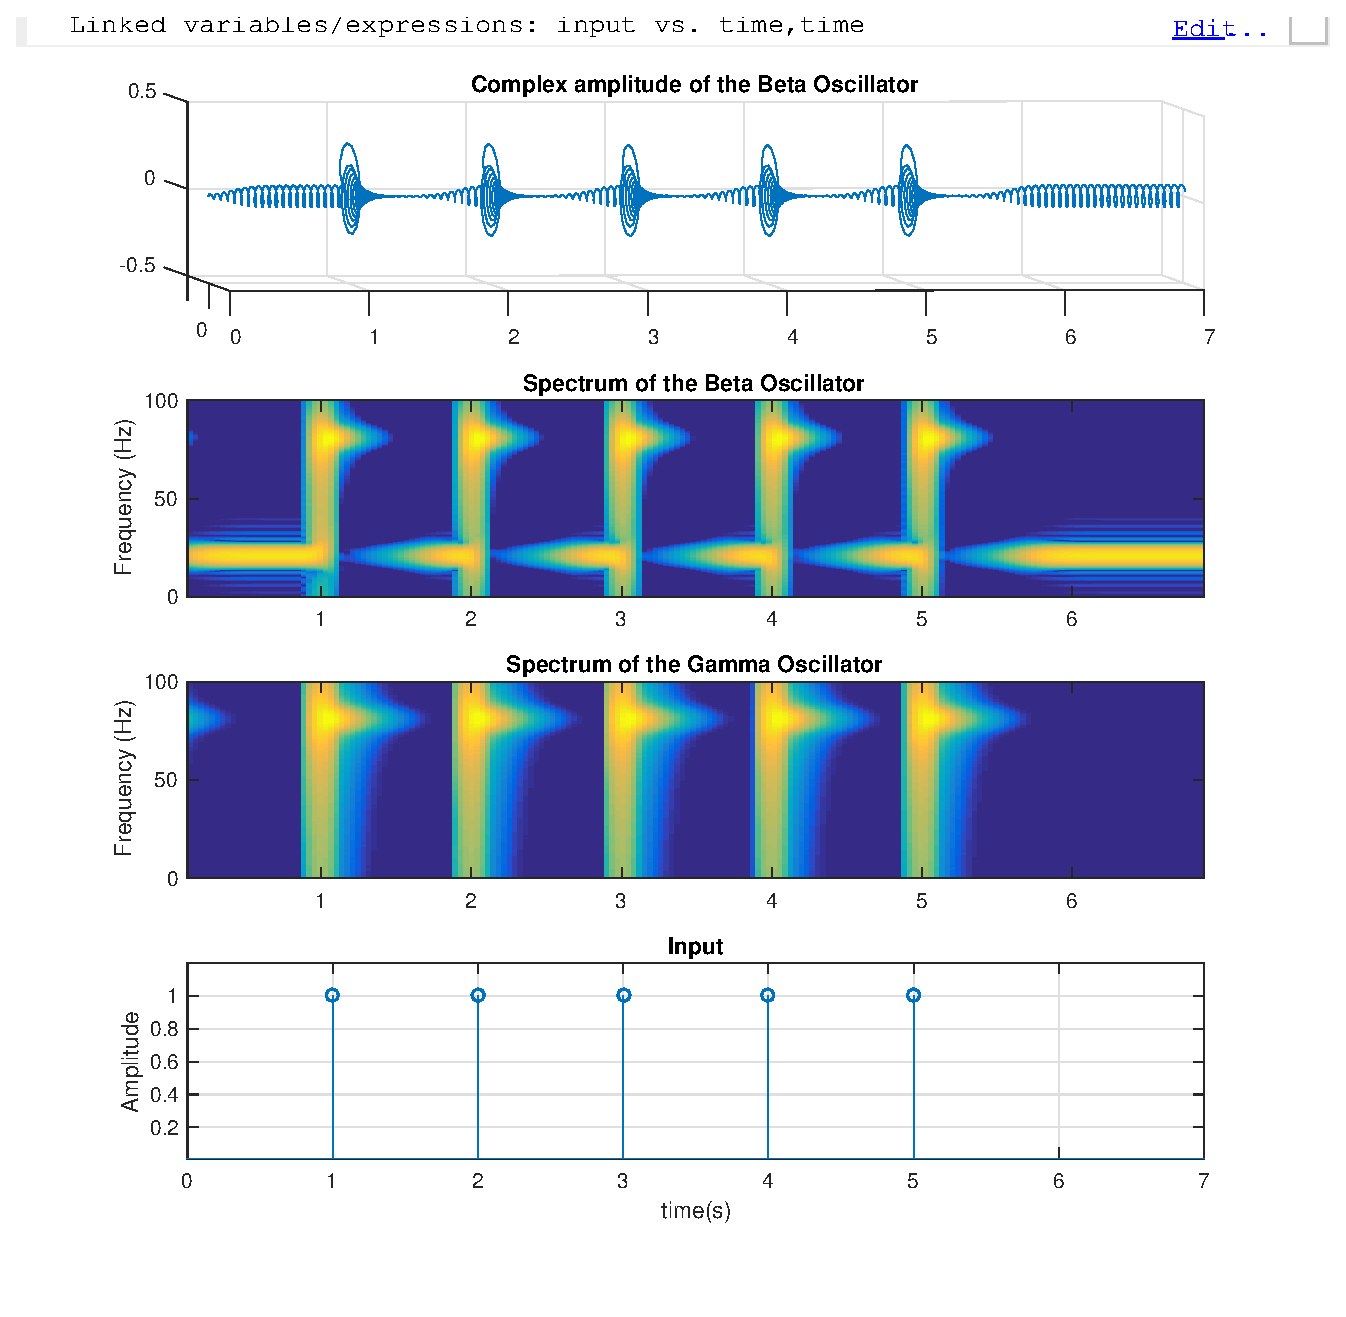
\includegraphics[width=\textwidth]{iso_stim}
        \caption{Results: [Row 1] Output. [Row 2] Output spectrogram. [Row 3] MC gamma bursting. [Row 4] MC impulse}
        \label{fig:system}
    \end{subfigure}
    ~ %add desired spacing between images, e. g. ~, \quad, \qquad, \hfill etc. 
    %(or a blank line to force the subfigure onto a new line)
%     \caption{(A) Output (B) MC/BG beta idling (C) MC gamma bursting (D) MC impulse}
\label{fig:animals}
\end{figure}

% \begin{figure}
% 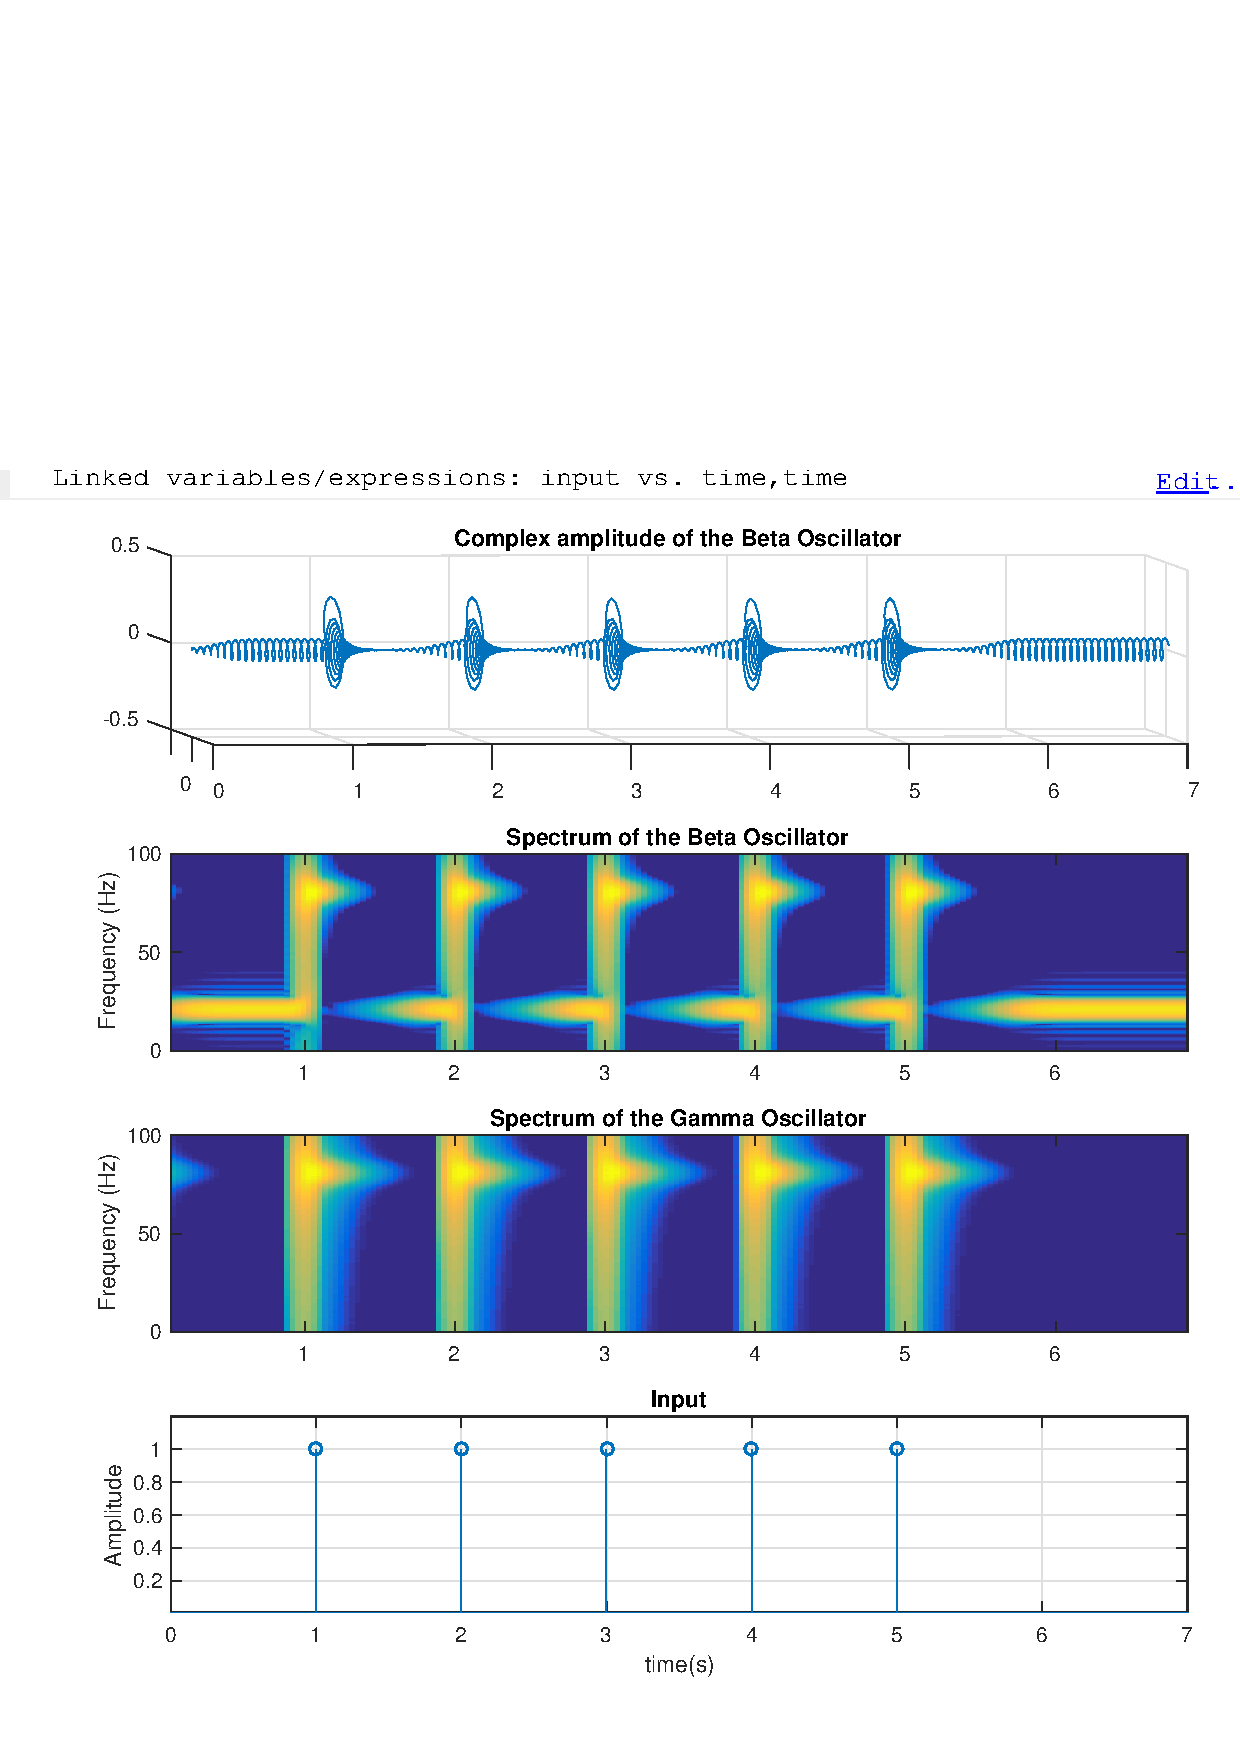
\includegraphics[width=.6\textwidth,right]{iso_stim.png}
% \label{fig:encoder}
% \end{figure}

%%%----------------------------------------------------------------- 
%%%%%%%%%%%%%%%%%%%%%%%%%%%%%%%%%%%%%%%
%%%%%%%%%%%%%%%% REFERENCES %%%%%%%%%%%%%%%%
%%%%%%%%%%%%%%%%%%%%%%%%%%%%%%%%%%%%%%%

{\bf References}\\
$\mathbf{[\,1\,]}$ Edward W Large, Felix V Almonte, and Marc J Velasco. A canonical model for
gradient frequency neural networks. Physica D: Nonlinear Phenomena, 239(12):905–911, 2010.\\
$\mathbf{[\,2\,]}$ Ji Chul Kim and Edward W. Large. Signal processing in periodically forced gradient frequency neural networks. Frontiers in Computational Neuroscience, 9:152, 2015.\\
$\mathbf{[\,3\,]}$ Takako Fujioka, Laurel J Trainor, Edward W Large, and Bernhard Ross. Beta and gamma rhythms in human auditory cortex during musical beat processing. Annals of the New York Academy of Sciences, 1169(1):89–92, 2009.\\
$\mathbf{[\,4\,]}$ Edward W Large, Jorge A Herrera, and Marc J Velasco. Neural networks for beat perception in musical rhythm. Frontiers in systems neuroscience, 9, 2015. \\
$\mathbf{[\,5\,]}$ John A Thompson, David Lanctin, Nuri Firat Ince, and Aviva Abosch. Clinical implications of local field potentials for understanding and treating movement disorders. Stereotactic and functional neurosurgery, 92(4):251–263, 2014.

% \bibliographystyle{apalike}
% {\footnotesize
% \bibliography{bibfile}}
% \bibliographystyle{unsrt}
% \bibliography{ref}

\end{document}